\documentclass{beamer}
\usepackage{beamerthemeshadow}
\usepackage[spanish]{babel}
\usepackage[utf8]{inputenc}
\usepackage[T1]{fontenc}
\usepackage{enumerate}
\usepackage{mathtools}
\usepackage{mathpazo}
\usepackage{amssymb}
\usepackage{stmaryrd}
\usepackage{lmodern}
\usepackage[font=scriptsize,justification=centering]{caption}

%\setbeamertemplate{theorems}[ams style] % numbered
\theoremstyle{definition}
\makeatletter
\setbeamertemplate{theorem begin}
{%
  \inserttheoremheadfont \bfseries
  \inserttheoremname \inserttheoremnumber
  \ifx\inserttheoremaddition\@empty\else\ (\inserttheoremaddition)\fi%
  :
  \normalfont
}
\setbeamertemplate{theorem end}{%
  % empty
}
\makeatother


\begin{document}
\title{Compresión: JPEG}
\author{Gabriel Thibeault y Gonzalo Ciruelos}
\date{13 de diciembre de 2017}


%\frame{\titlepage}

\section{Introducción}
\frame{\frametitle{El trabajo}

Este trabajo se basa en la realización de una implementación del algoritmo
de compresión usado por el estándar de JPEG.

\hspace{1cm}

JPEG es un método común de compresión con pérdida para imágenes digitales.
El grado de compresión puede ajustarse, permitiendo un compromiso entre
tamaño y calidad de la imágen resultante.

\hspace{2cm}

El trabajo en el cual basamos nuestra implementación es

\begin{center}
  Gregory K. Wallace. The JPEG still picture compression standard.
  \emph{IEEE Transactions on Consumer Electronics}, 38(1):XVIII--XXXIV, 1992.
\end{center}
}

\frame{\frametitle{DCT}

La DCT bidimensional no es más que aplicar la unidimensional por filas y luego por columnas.
La fórmula para 8x8 a continuación puede generalizarse:

\footnotesize{
\begin{equation*}
    F(u, v) = \frac{C(u)C(v)}{4} \sum\limits_{x = 0}^{7}
    \bigg(\sum\limits_{y = 0}^{7} f(x, y) 
    cos\Big(\frac{(2x + 1)u\pi}{16}\Big)\bigg)
    cos\Big(\frac{(2y + 1)v\pi}{16}\Big)
\end{equation*}

La anti-transformada:

\begin{equation*}
    f(x, y) =  \sum\limits_{u = 0}^{7}
    \bigg(\sum\limits_{v = 0}^{7} \frac{C(u)C(v)}{4}F(u, v) 
    cos\Big(\frac{(2x + 1)u\pi}{16}\Big)\bigg)
    cos\Big(\frac{(2y + 1)v\pi}{16}\Big)
\end{equation*}
\begin{equation*}
    C(t) :=
    \begin{cases}
        \frac{1}{\sqrt{2}} &\quad\text{si } t = 0 \\
        1                  &\quad\text{si } t \neq 0
    \end{cases}
\end{equation*}
}}

\frame{\frametitle{Cuantización}

\small{La cuantización es el paso de JPEG que introduce pérdidas.}

\begin{equation*}
    F^Q(u, v) = Round\Big(\frac{F(u, v)}{Q(u, V)}\Big)
\end{equation*}

\footnotesize{La operación inversa:}

\begin{equation*}
    F'(u, v) = F^Q(u, v)Q(u, V)
\end{equation*}

\footnotesize{$Q$ es una matriz fija multiplicada por una constante de cuantización $q_{AC}$.
El primer coeficiente, $F(0, 0)$ puede ser cuantizado distintamente del resto: $Q(0, 0) = 16 * q_{DC}$.}

\begin{equation*}
    Q = q_{AC} * 
\begin{bmatrix}
16 &  11  & 10  & 16  & 24  & 40   &  51  &  61  \\ %\hline
12 &  12  & 14  & 19  & 26  & 58   &  60  &  55  \\ %\hline
14 &  13  & 16  & 24  & 40  & 57   &  69  &  56  \\ %\hline
14 &  17  & 22  & 29  & 51  & 87   &  80  &  62  \\ %\hline
18 &  22  & 37  & 56  & 68  & 109  &  103 &  77  \\ %\hline
24 &  35  & 55  & 64  & 81  & 104  &  113 &  92  \\ %\hline
49 &  64  & 78  & 87  & 103 &  121 &  120 &  101 \\ %\hline
72 &  92  & 95  & 98  & 112 &  100 &  103 &  99  \\ %\hline
\end{bmatrix}
\end{equation*}
}

\frame{\frametitle{Codificación de Huffman}

\begin{enumerate}
  \item Diferencial de $DC$s.
  \item Representación zig-zag.
  \item Run lenghts.
  \item Codificación de Huffman usando esos pares como los símbolos del lenguaje.
\end{enumerate}

\begin{center}
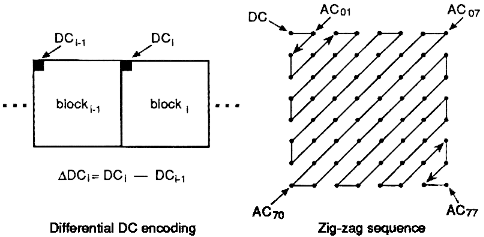
\includegraphics[width=5cm]{images/huffman.png}
\end{center}

\[
  [10, 1, 1, 0, 0, 0, 0, 2, 1, 0, 0, 1, 0, 0, 0, 0]
\]
\[
  \to [(0, 10), (0, 1), (0, 1), (4, 2), (0, 1), (2, 1)]
\]
}

\frame{\frametitle{Imágenes a Color}

Para comprimir una imagen en $RGB$ se convierte al espacio $Y'C_bC_r$.
El componente $Y'$ es análogo a la intensidad en $HSI$, mientras que $C_b$ y $C_r$ mantienen información de color (la diferencia de azul y rojo respecto de $Y'$).

\hspace{1cm}

Luego de transformar, el componente $Y'$ es comprimido como se detalló previamente.
Se toman bloques de tamaño $M_c \times M_c$ y se promedian $C_b$ y $C_r$ para cada bloque.
}

\frame{\frametitle{Imágenes a Color: ejemplo}
\begin{center}
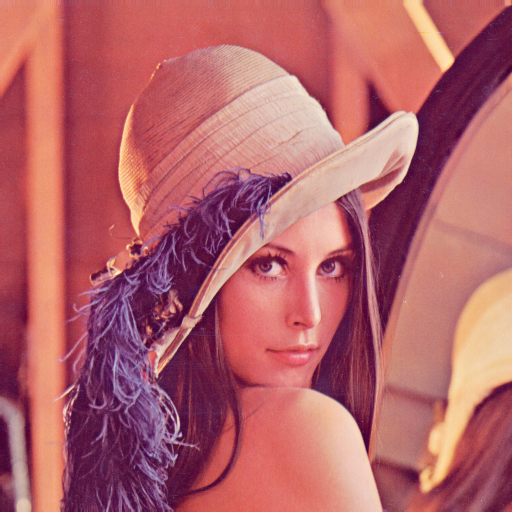
\includegraphics[width=6cm]{images/lenaColor.png} 
\par Imagen original a color.
\end{center}
}
\frame{\frametitle{Imágenes a Color: ejemplo}
\begin{center}
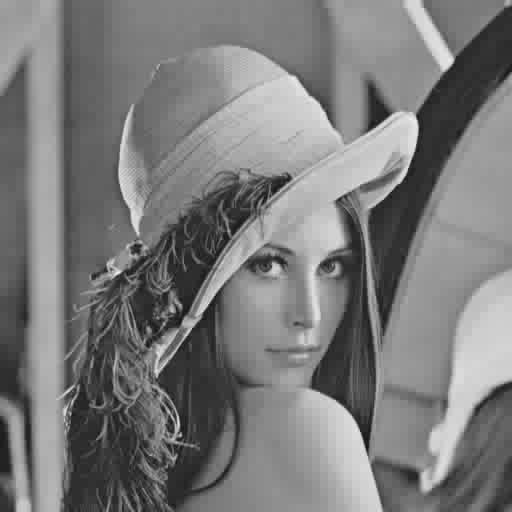
\includegraphics[width=5cm]{images/lenaY_comp.png} 

\includegraphics[width=5cm]{images/lenaCbCr_comp.png}
\par Componente $Y'$ (izquierda) y $C_b, C_r$ (derecha).
\end{center}
}
\frame{\frametitle{Imágenes a Color: ejemplo}
\begin{center}
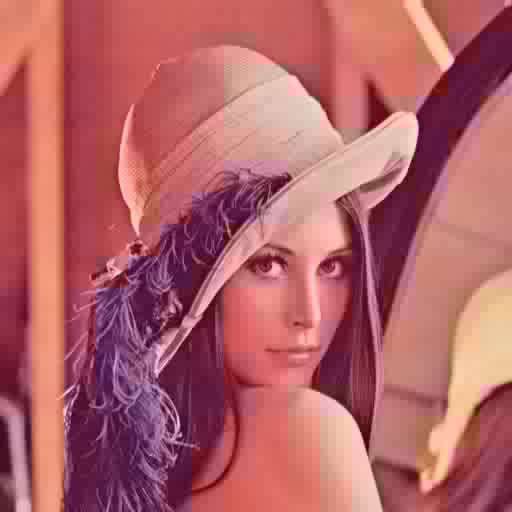
\includegraphics[width=6cm]{images/lena_comp.png}
\par Imagen tras descomprimir.
\end{center}
}

\frame{\frametitle{Análisis cuantitativo (grises): Tamaño del bloque}
\begin{center}
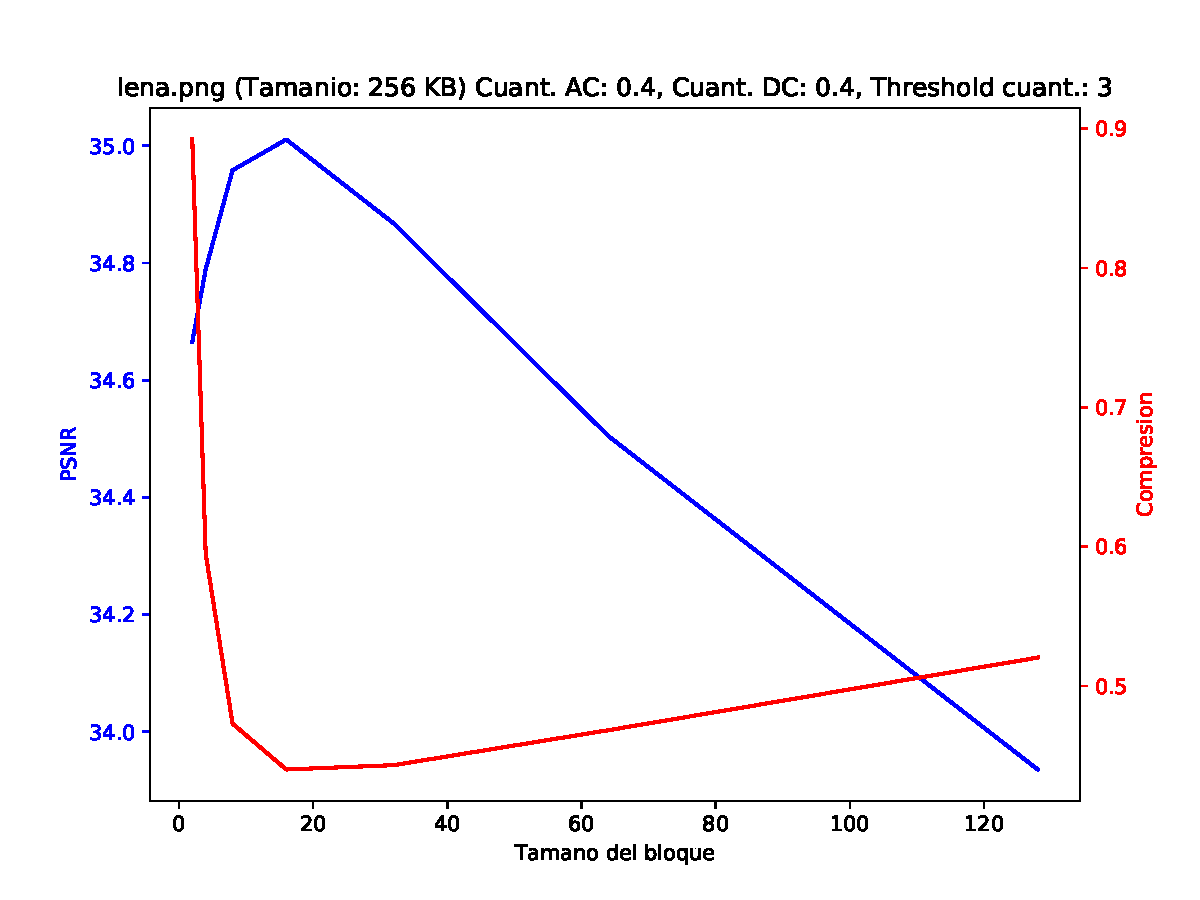
\includegraphics[width=10cm]{images/quant-grey-m.pdf}
\end{center}
}

\frame{\frametitle{Análisis cuantitativo (grises): Cuantización de DC}
\begin{center}
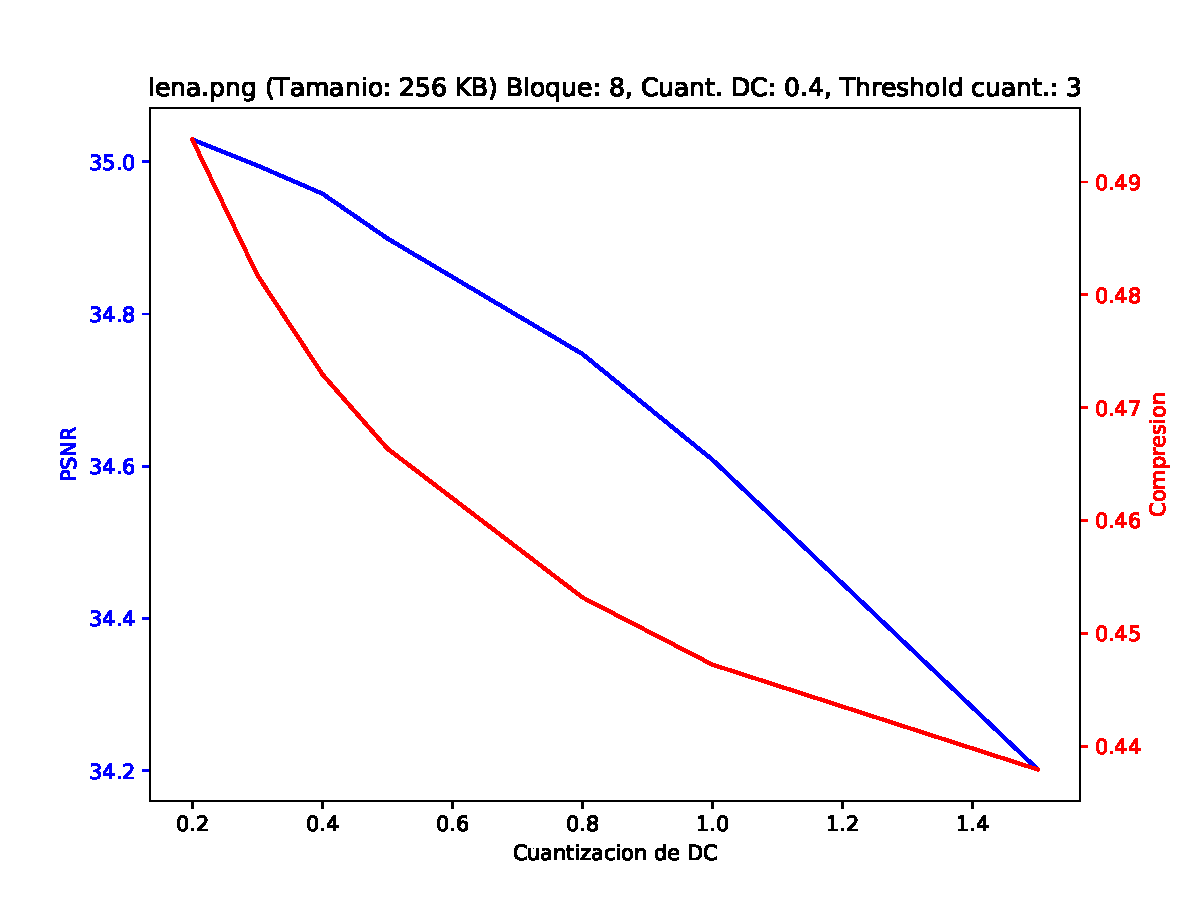
\includegraphics[width=10cm]{images/quant-grey-qdc.pdf}
\end{center}
}

\frame{\frametitle{Análisis cuantitativo (grises): Cuantización de AC}
\begin{center}
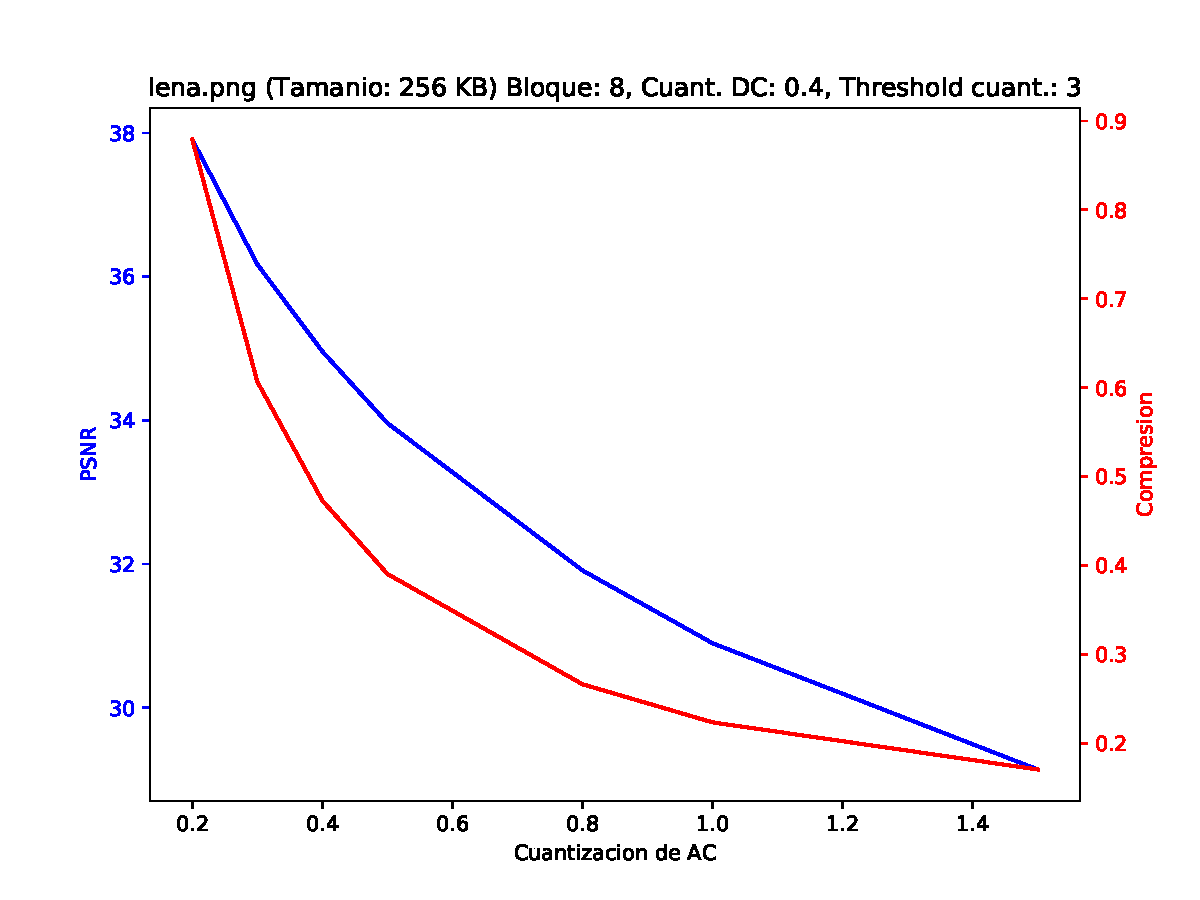
\includegraphics[width=10cm]{images/quant-grey-qac.pdf}
\end{center}
}

\frame{\frametitle{Análisis cuantitativo (grises): Threshold de cuantización}
\begin{center}
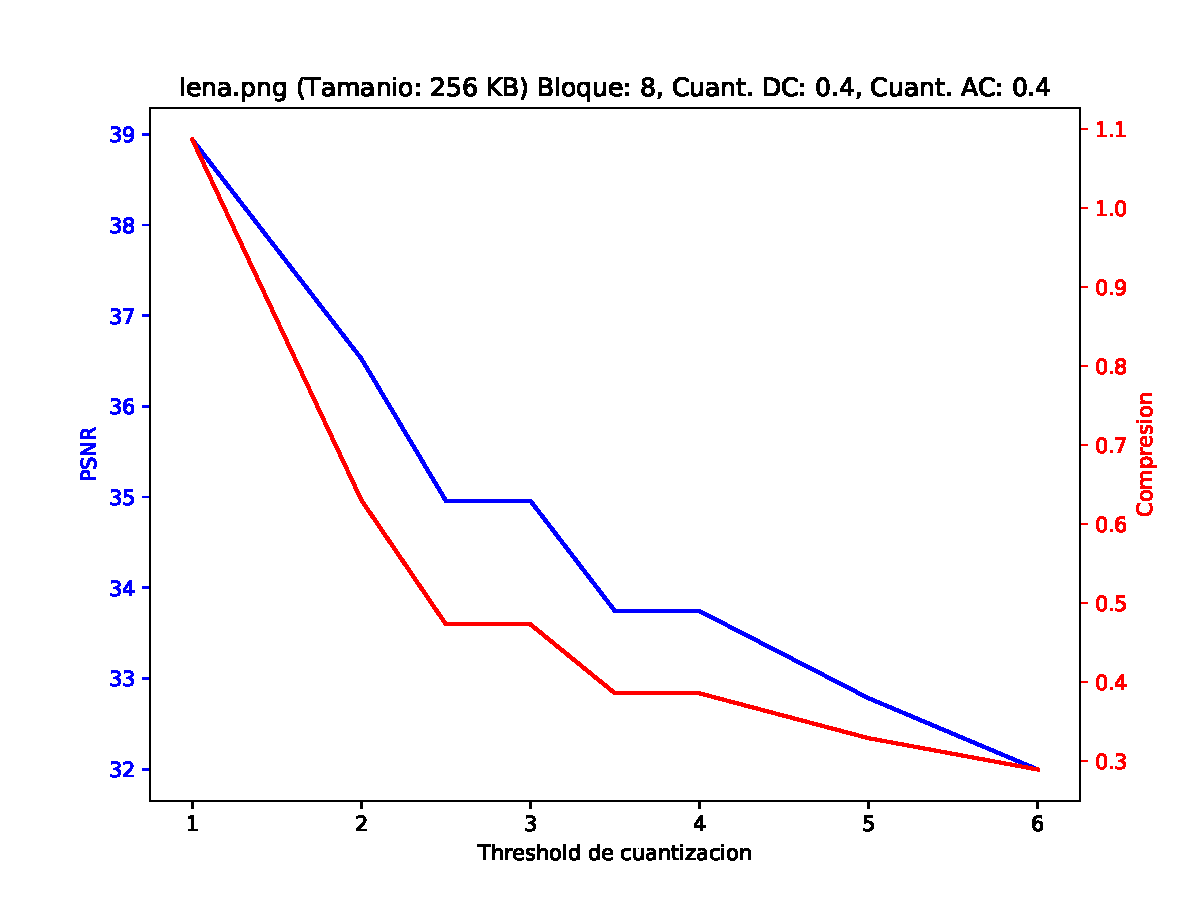
\includegraphics[width=10cm]{images/quant-grey-u.pdf}
\end{center}
}

\frame{\frametitle{Análisis cuantitativo (RGB): Tamaño del bloque}
\begin{center}
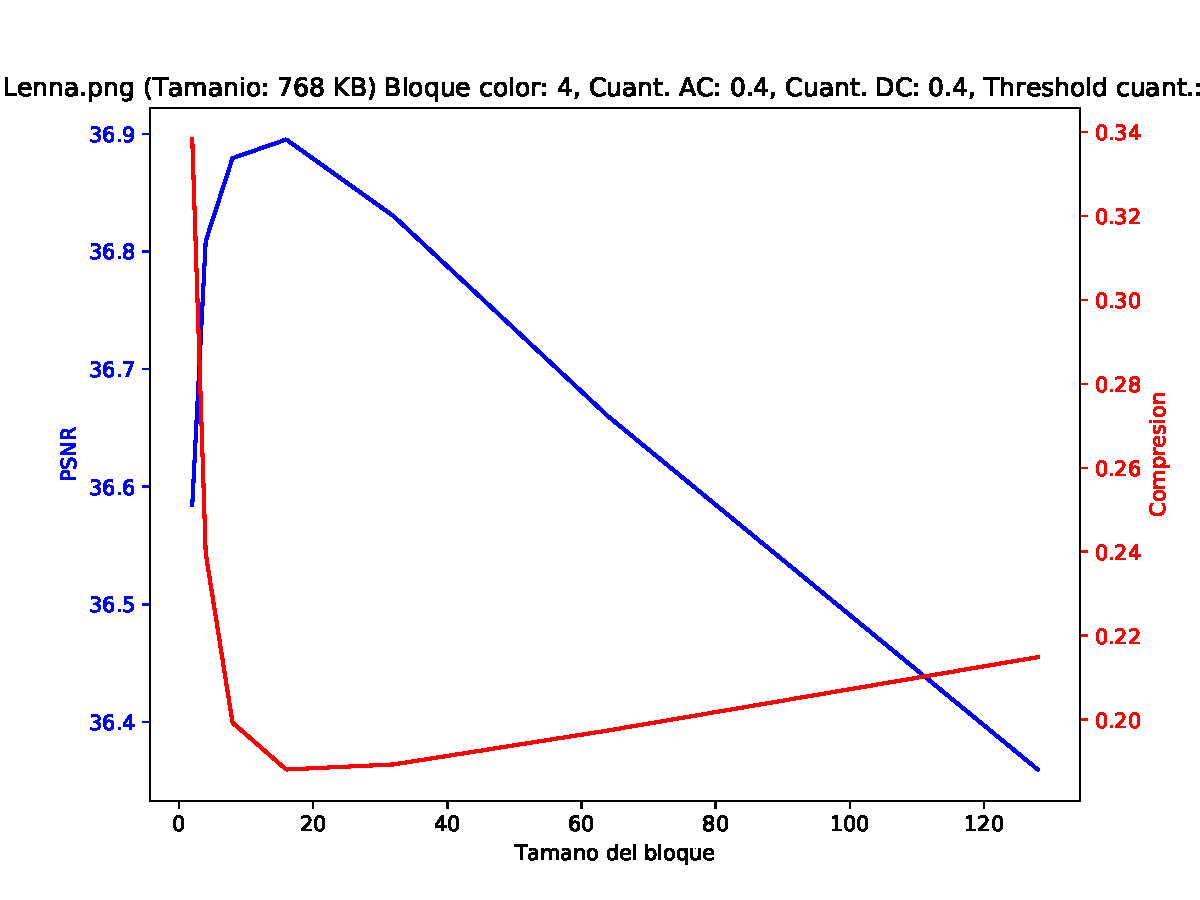
\includegraphics[width=10cm]{images/quant-rgb-m.pdf}
\end{center}
}

\frame{\frametitle{Análisis cuantitativo (RGB): Tamaño del bloque de color}
\begin{center}
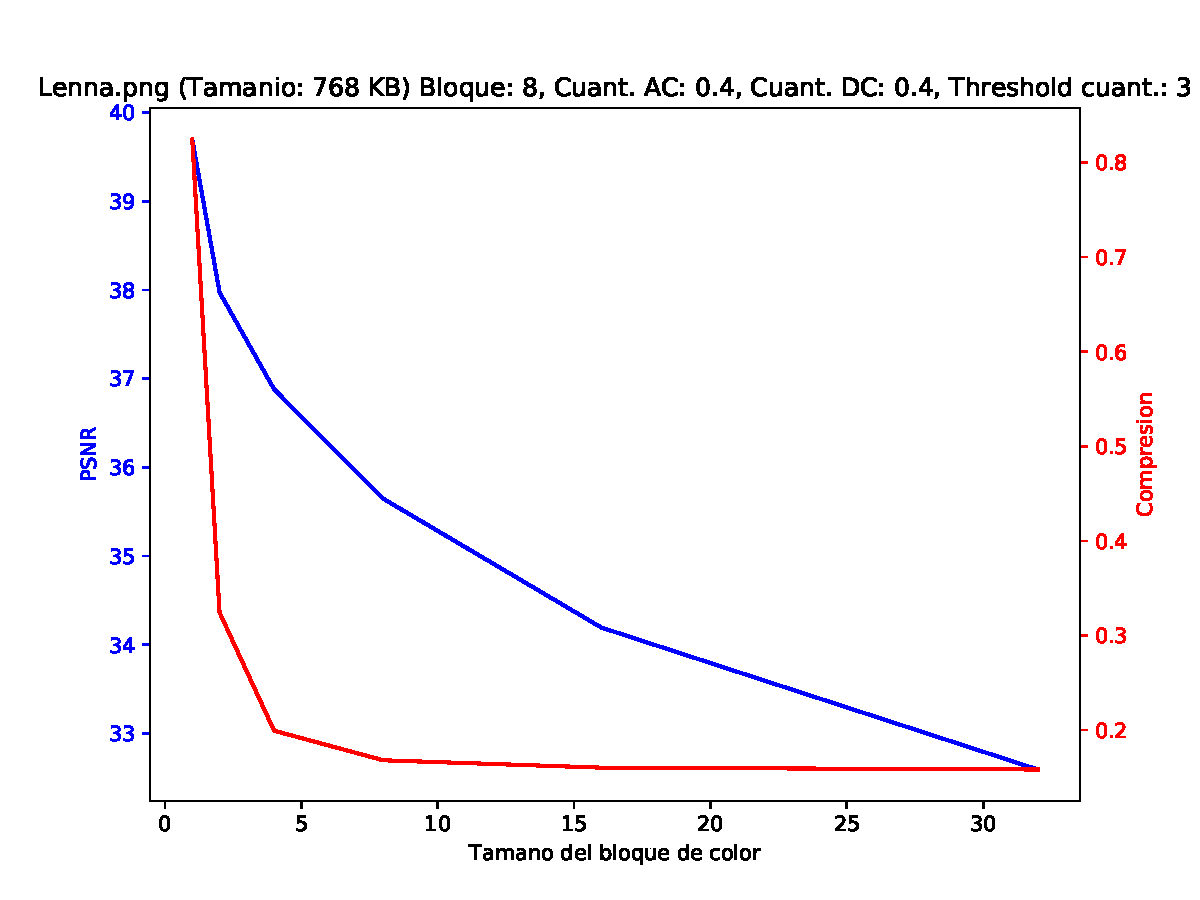
\includegraphics[width=10cm]{images/quant-rgb-mcolor.pdf}
\end{center}
}

\frame{\frametitle{Análisis cuantitativo (RGB): Cuantización de DC}
\begin{center}
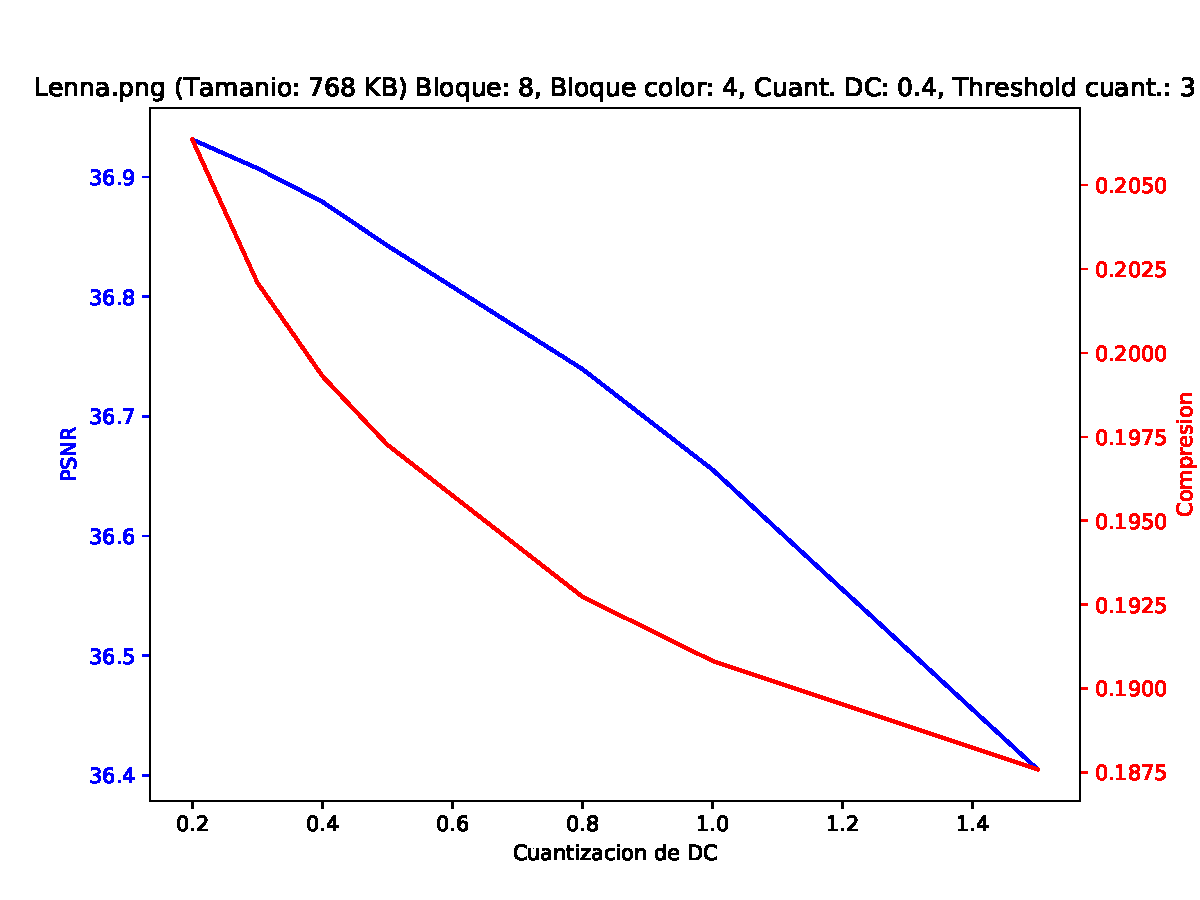
\includegraphics[width=10cm]{images/quant-rgb-qdc.pdf}
\end{center}
}

\frame{\frametitle{Análisis cuantitativo (RGB): Cuantización de AC}
\begin{center}
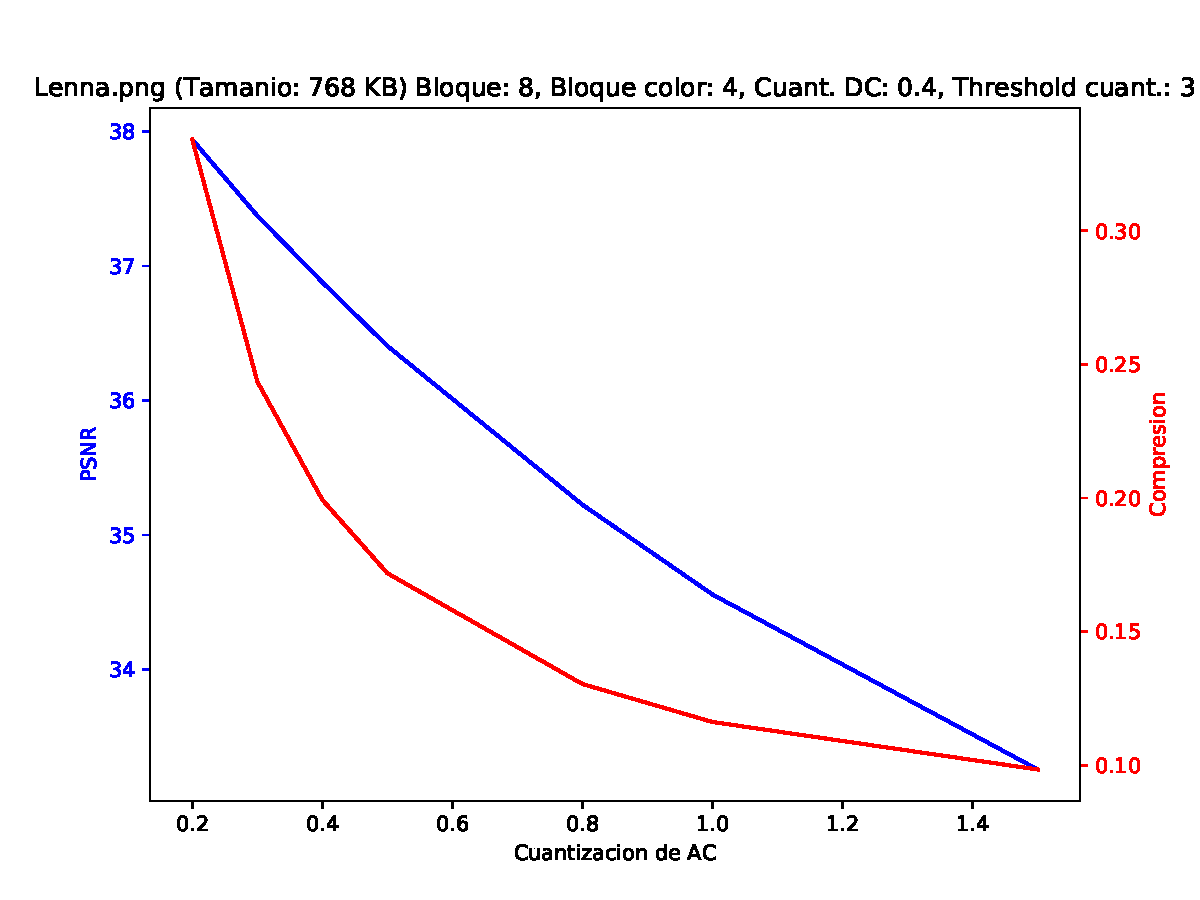
\includegraphics[width=10cm]{images/quant-rgb-qac.pdf}
\end{center}
}

\frame{\frametitle{Análisis cuantitativo (RGB): Threshold de cuantización}
\begin{center}
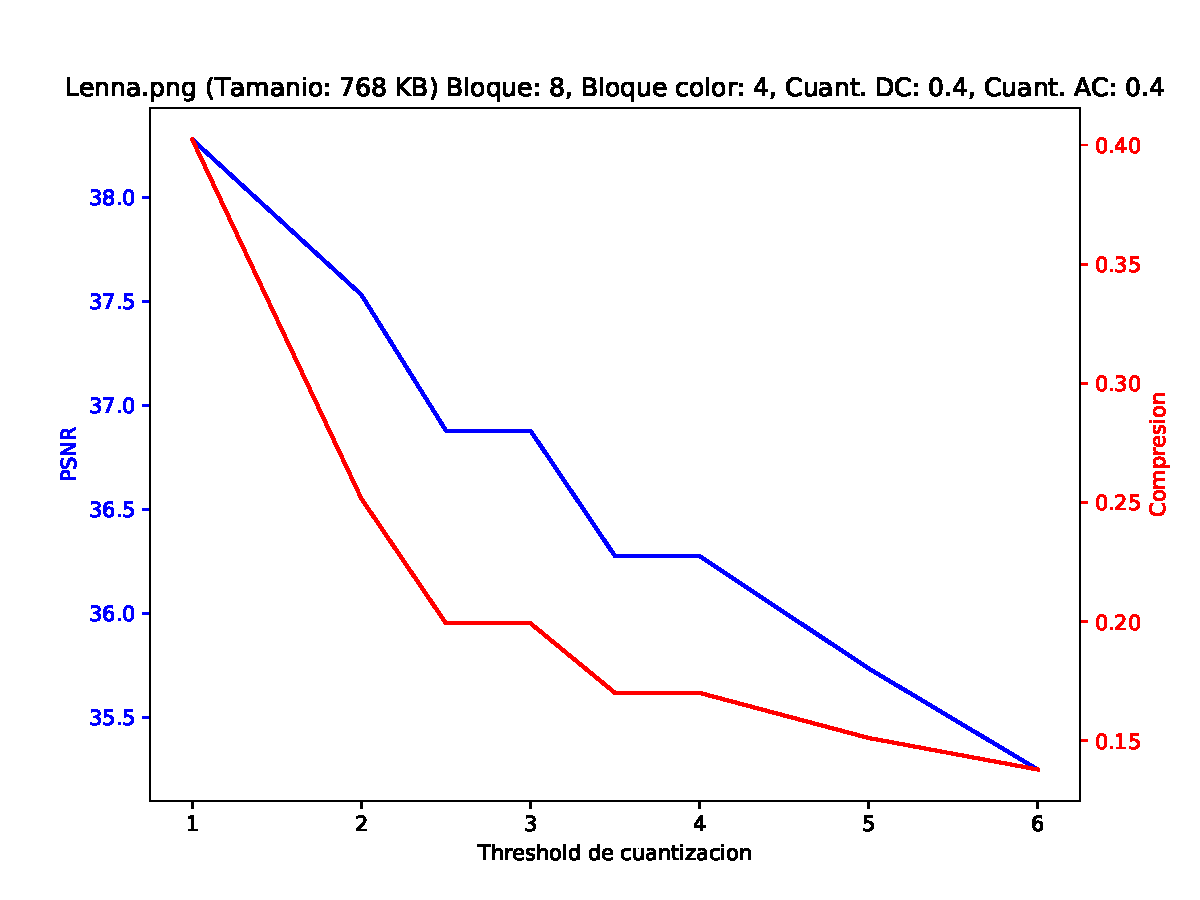
\includegraphics[width=10cm]{images/quant-rgb-u.pdf}
\end{center}
}

\frame{\frametitle{Análisis cuantitativo: parámetros óptimos (rangos)}
\begin{itemize}
  \item Tamaño del bloque: $8 \times 8$ -- $16 \times 16$.
  \item Tamaño del bloque de color: $2 \times 2$ -- $4 \times 4$.
  \item Cuantización del DC: $1.0$ -- $1.2$.
  \item Cuantización del AC: $0.2$ -- $0.5$.
  \item Threshold de cuantización $1$ -- $3$.
\end{itemize}
}



\frame{\frametitle{Análisis cualitativo (grises)}
\begin{center}
    \includegraphics[width=6cm]{images/{16-16-3-3-4}.png}
    \par $M = 16; q_{DC} = 3; q_{AC} = 3; U = 4$.
    \par Severo \textit{blocking}.
\end{center}
}

\frame{\frametitle{Análisis cualitativo (grises)}
\begin{center}
    \includegraphics[width=6cm]{images/{32-32-.5-.5-2}.png}
    \par $M = 32; q_{DC} = 0.5; q_{AC} = 0.5; U = 2$. 
    \par Bien condicionada.
\end{center}
}

\frame{\frametitle{Análisis cualitativo (grises)}
\begin{center}
    \includegraphics[width=6cm]{images/{32-32-1.5-1.5-2}.png}
    \par $M = 32; q_{DC} = 1.5; q_{AC} = 1.5; U = 2$. 
    \par Ligero \textit{blocking} y \textit{ringing}.
\end{center}
}

\frame{\frametitle{Análisis cualitativo (grises)}
\begin{center}
    \includegraphics[width=6cm]{images/{32-32-1.5-1.5-4}.png}
    \par $M = 32; q_{DC} = 1.5; q_{AC} = 1.5; U = 2$. 
    \par Ligero \textit{blocking} y \textit{ringing}.
\end{center}
}

\frame{\frametitle{Análisis cualitativo (grises)}
\begin{center}
    \includegraphics[width=5cm]{images/{8-8-.5-.5-2}.png}
    \includegraphics[width=5cm]{images/{32-32-.5-.5-2}.png}
    \par Se observa menor \textit{blocking} a pesar de aumentar 16 veces el tamaño de los 
    bloques en la imagen de la derecha.
\end{center}
}

\frame{\frametitle{Análisis cualitativo (color)}
\begin{center}
    \includegraphics[width=6cm]{images/{lena_comp}.png}
    \par \textit{Blocking} por color y gris. Artifacts de color por bloques cruzando bordes.
\end{center}
}

\frame{\frametitle{Análisis cualitativo (color)}
\begin{center}
    \includegraphics[width=6cm]{images/{32-32-2-2-2}.png}
    \par \textit{Blocking} por color y gris. \textit{Ringing}.
\end{center}
}

\frame{\frametitle{Análisis cualitativo (color)}
\begin{center}
    \includegraphics[width=6cm]{images/{8-32-.5-.5-1}.png}
    \par Artifacts de \textit{blocking} debido a superficie diagonal.
\end{center}
}

\frame{
\huge
\begin{center}
¿Preguntas?
\end{center}
}

\end{document}
